%\addcontentsline{toc}{chapter}{Development Process}
\chapter{Design}

%You should concentrate on the more important aspects of the design. It is essential that an overview is presented before going into detail. As well as describing the design adopted it must also explain what other designs were considered and why they were rejected.
%
%The design should describe what you expected to do, and might also explain areas that you had to revise after some investigation.
%
%Typically, for an object-oriented design, the discussion will focus on the choice of objects and classes and the allocation of methods to classes. The use made of reusable components should be described and their source referenced. Particularly important decisions concerning data structures usually affect the architecture of a system and so should be described here.
%
%How much material you include on detailed design and implementation will depend very much on the nature of the project. It should not be padded out. Think about the significant aspects of your system. For example, describe the design of the user interface if it is a critical aspect of your system, or provide detail about methods and data structures that are not trivial. Do not spend time on long lists of trivial items and repetitive descriptions. If in doubt about what is appropriate, speak to your supervisor.
% 
%You should also identify any support tools that you used. You should discuss your choice of implementation tools - programming language, compilers, database management system, program development environment, etc.
%
%Some example sub-sections may be as follows, but the specific sections are for you to define. 

\section{Overall Architecture}
\begin{figure}[H]
	\centering
	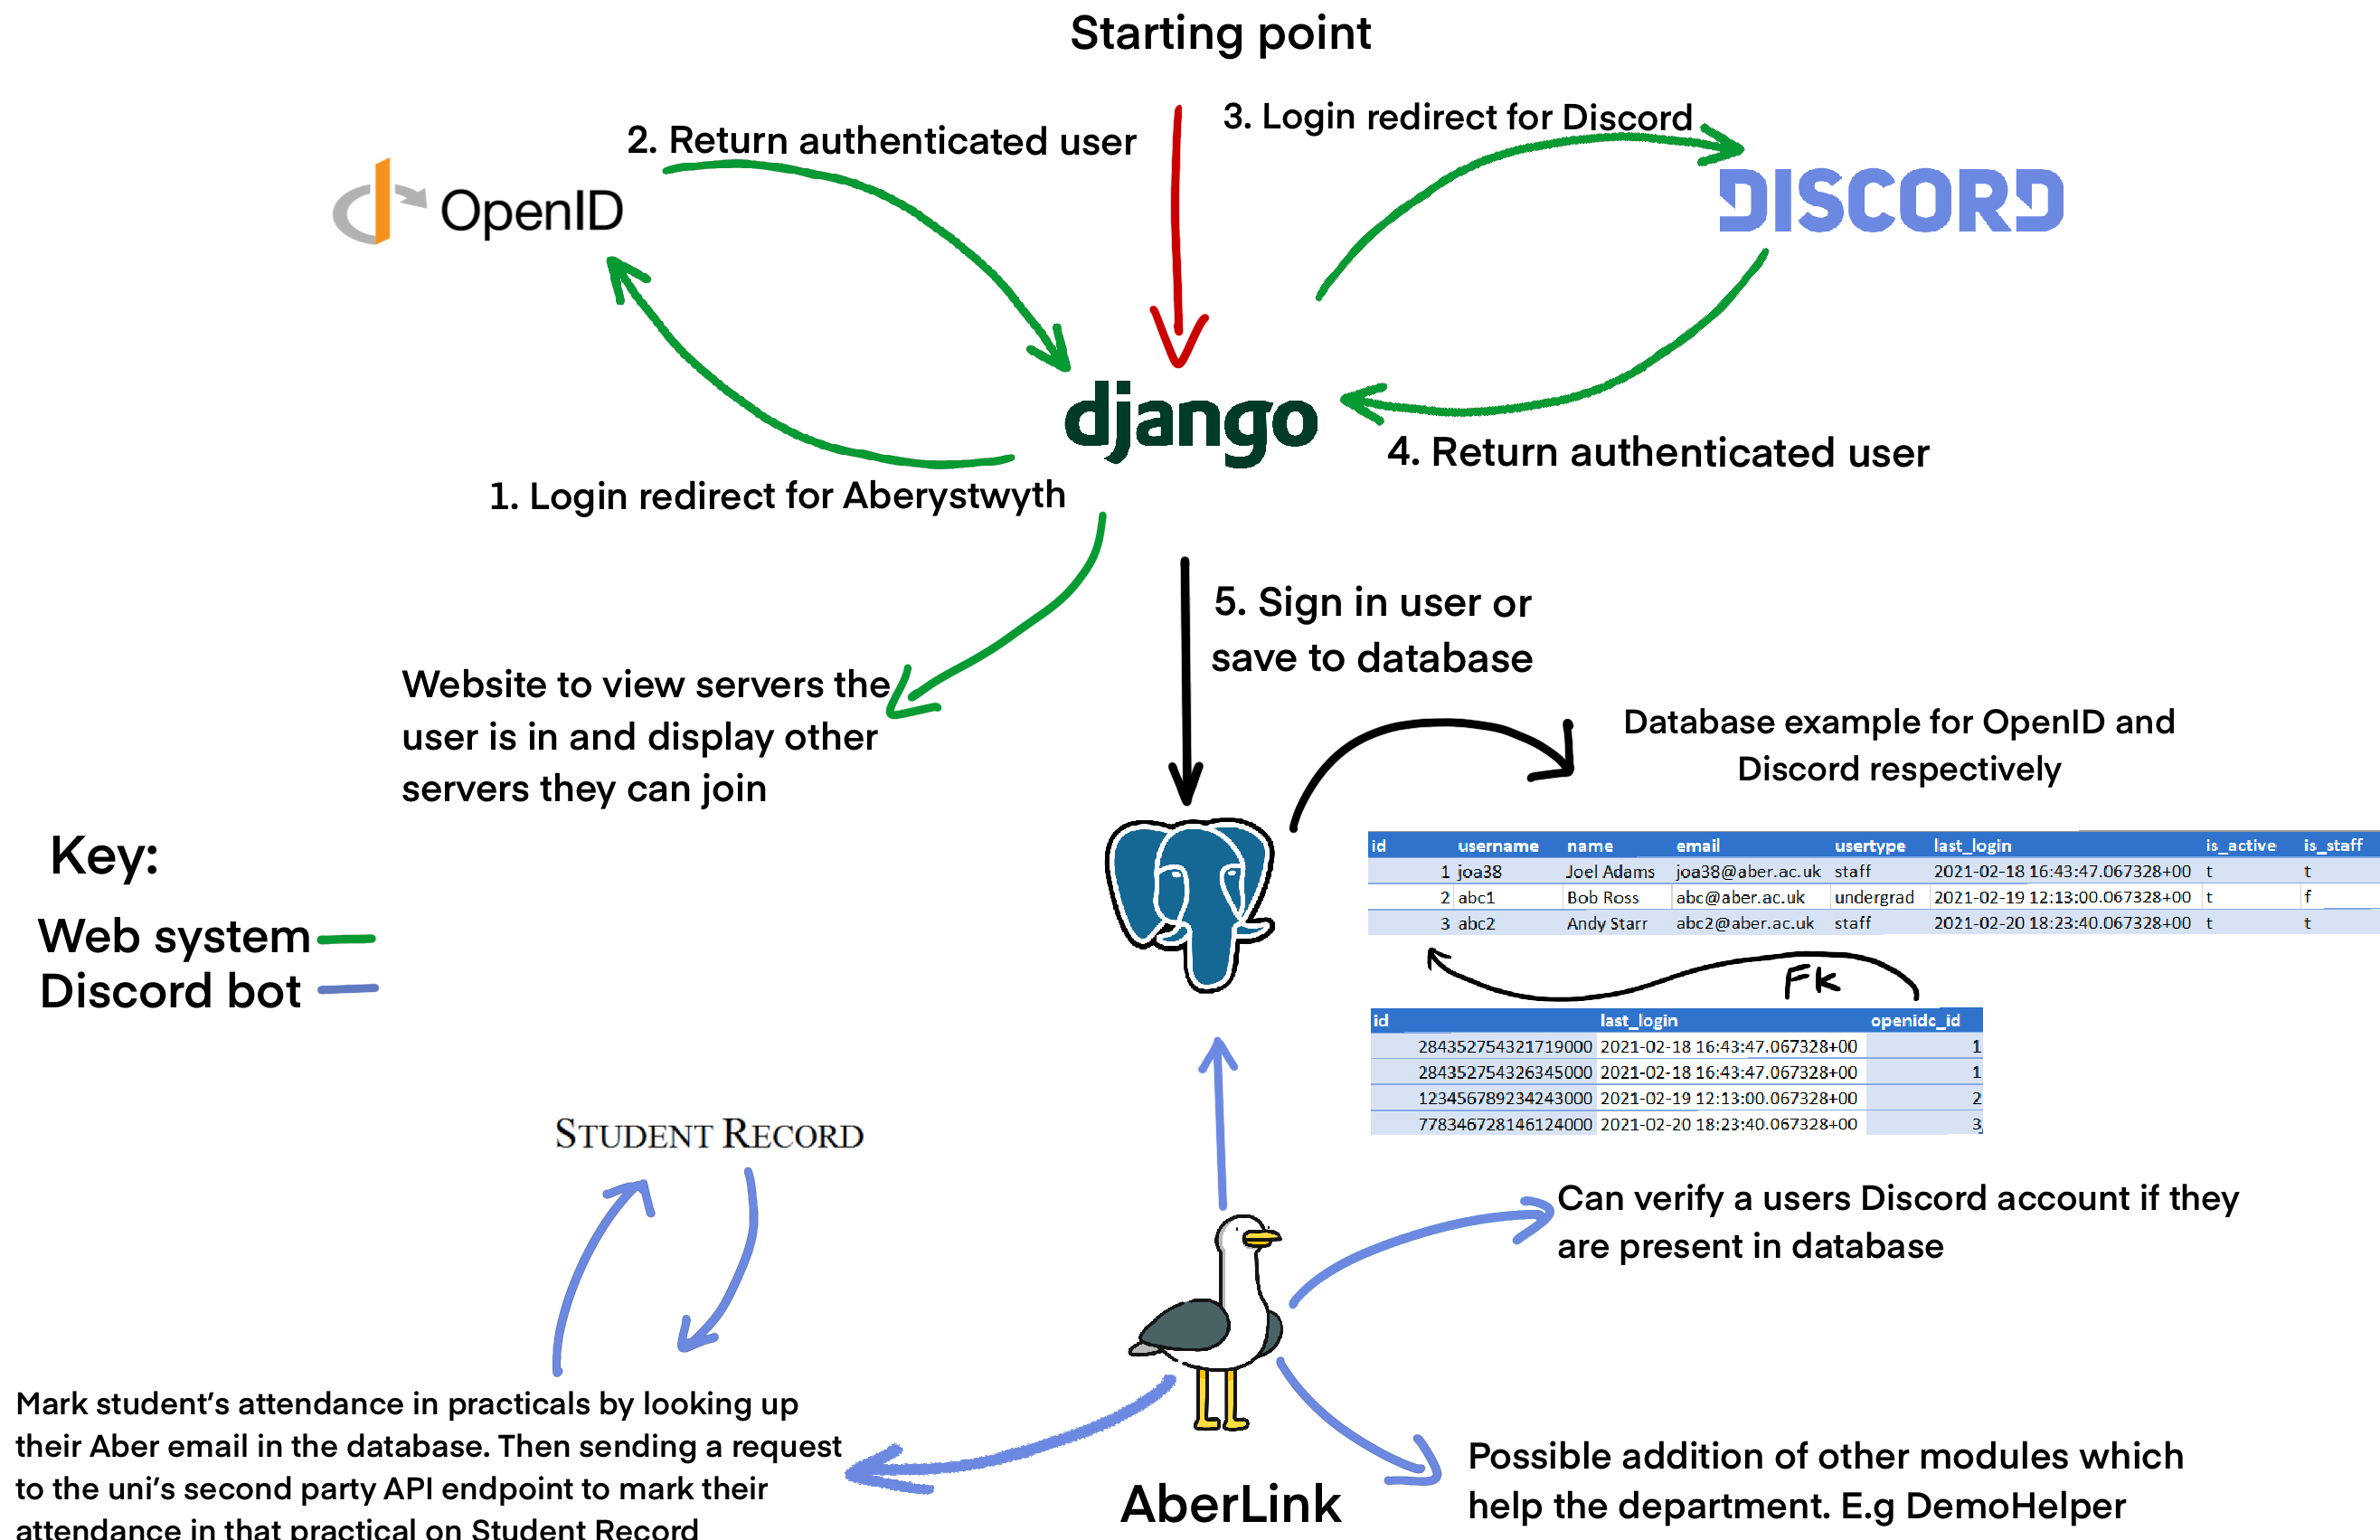
\includegraphics[width=1\linewidth]{Figures/aberlink-flowchart-3}
	\caption{Architecture diagram of the overall system}
	\label{fig:architecture}
\end{figure}

Below is a diagram displaying the overall file structure used for the project and was inspired by the second year group project. It has a config folder which describes how to setup the whole project, a folder called dev which contains all of the projects spikework and a folder called docs that contains the latex documents required for this project such as this document. There is also a folder called src that contains two sub folders AberLinkAuthentication and AberLinkDiscord. These two folders are in charge of the website and Discord bot respectively and have been split up as the underlying architecture for each one is vastly different and helps greatly with code maintainability.

\begin{figure}[H]
\begin{forest}
	for tree={
		font=\ttfamily,
		grow'=0,
		child anchor=west,
		parent anchor=south,
		anchor=west,
		calign=first,
		edge path={
			\noexpand\path [draw, \forestoption{edge}]
			(!u.south west) +(7.5pt,0) |- node[fill,inner sep=1.25pt] {} (.child anchor)\forestoption{edge label};
		},
		before typesetting nodes={
			if n=1
			{insert before={[,phantom]}}
			{}
		},
		fit=band,
		before computing xy={l=15pt},
	}
	[aberlink
	[config]
	[dev]
	[docs]
	[src
	[AberLinkAuthentication]
	[AberLinkDiscord]
	]
	]
\end{forest}
\caption{Tree diagram showing overall folder structure}
\label{fig:architecture-tree}
\end{figure}

\section{Website Architecture and Design}
\begin{figure}[H]
	\centering
	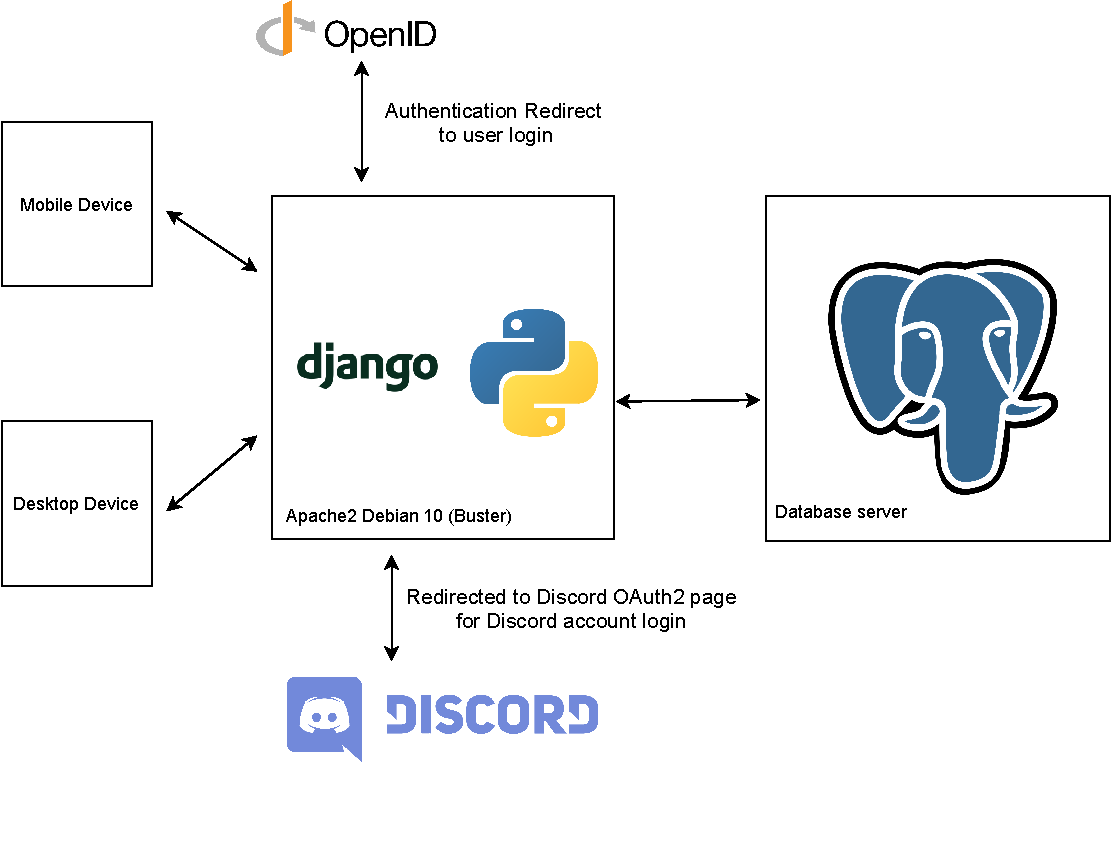
\includegraphics[width=1\linewidth]{Figures/Architecture-website}
	\caption{Architecture diagram of website}
	\label{fig:architecture-web}
\end{figure}

The website is built using the Python framework Django \cite{Django}. This framework has been used to generate a template of the code required and only requires minimal tweaking to setup. When you visit the website you then get redirected to the OpenID Connect \cite{OpenID} authentication framework which helps to prevent unwanted access by users who aren't permitted to view the website. Once authenticated the users data is then saved to the database and they can then add Discord accounts by using the button displayed on the screen. This then redirects them to Discord's OAuth2 authentication page and once they've logged in with a discord account then it redirects them back to the my website and saves that information to the database as well. I have included a flow chart below to explain the process.

\begin{figure}[H]
	\centering
	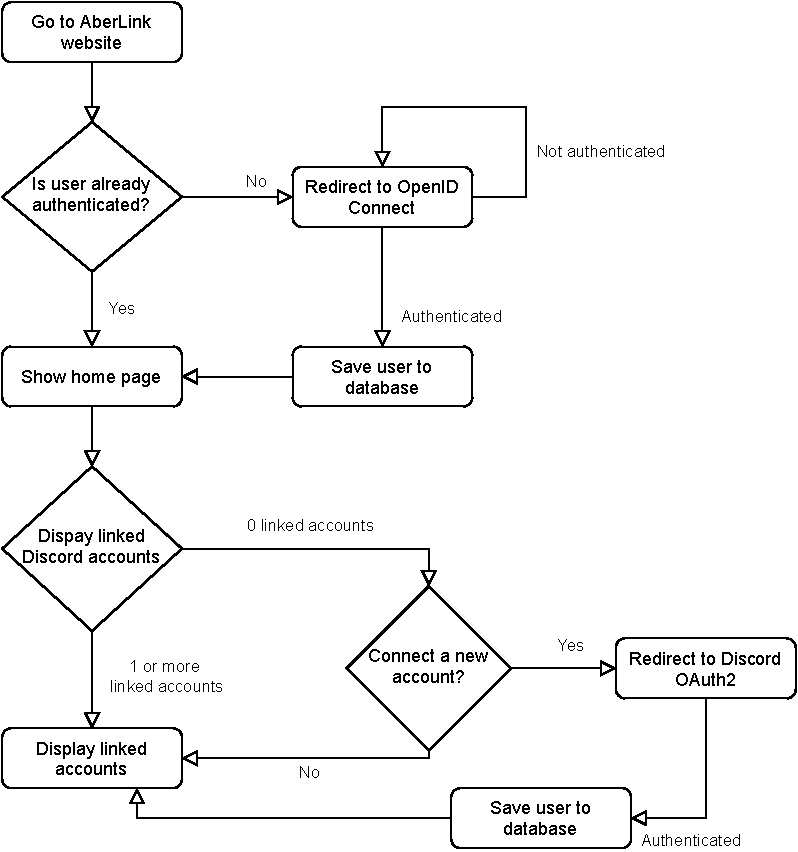
\includegraphics[width=0.8\linewidth]{Figures/website-flowchart}
	\caption{Website flowchart for authentication of accounts}
	\label{fig:architecture-web-flow}
\end{figure}

The website can be found here \href{https://mmp-joa38.dcs.aber.ac.uk/}{https://mmp-joa38.dcs.aber.ac.uk/} and is only accessible over VPN.

\section{Discord Bot Architecture and Design}
\begin{figure}[H]
	\centering
	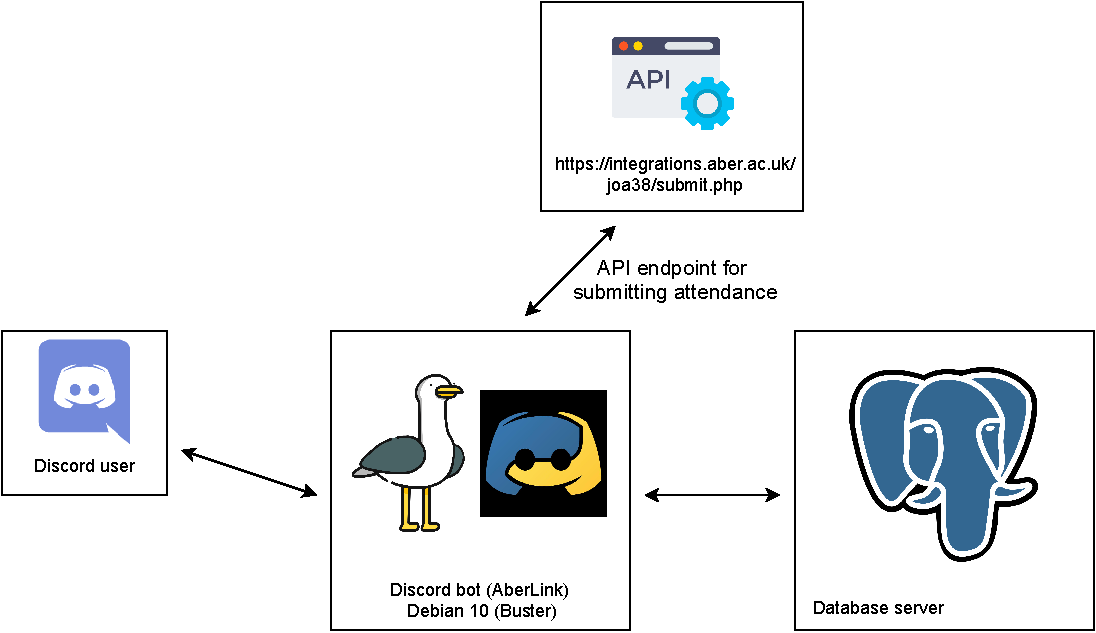
\includegraphics[width=0.9\linewidth]{Figures/Architecture-discord}
	\caption{Architecture diagram of Discord bot}
	\label{fig:architecture-dis}
\end{figure}

The Discord bot (AberLink) is interactable through the Discord application available on mobile, desktop and website. AberLink has many commands which can be easily found by typing the !help command in Discord on a server where the bot is present. The basic premise however is that it can access the database to retrieve information about a user; it never saves any information to the database however. The file structure goes as follows:

\begin{figure}[H]
\begin{forest}
	for tree={
		font=\ttfamily,
		grow'=0,
		child anchor=west,
		parent anchor=south,
		anchor=west,
		calign=first,
		edge path={
			\noexpand\path [draw, \forestoption{edge}]
			(!u.south west) +(7.5pt,0) |- node[fill,inner sep=1.25pt] {} (.child anchor)\forestoption{edge label};
		},
		before typesetting nodes={
			if n=1
			{insert before={[,phantom]}}
			{}
		},
		fit=band,
		before computing xy={l=15pt},
	}
	[AberLinkDiscord
	[AberLink.py]
	[Pipfile]
	[.env]
	[cogs
		[\_\_init\_\_.py]
		[db.py]
		[here.py]
		[utilities.py]
		[verify.py]
	]
	]
\end{forest}
\caption{Tree diagram showing Discord file structure}
\label{fig:dis-tree}
\end{figure}

As seen above in the file structure the main file that is used to run the program called AberLink.py, initialising the bot instance and loading all the files from the cogs folder. Discord.py \cite{discord.py} uses a smart system where code is not written into the main file (in this case AberLink) but instead separated out into components or 'cogs' as they're called here. The .env file is used to to store sensitive variables such as the Discord token required to run the bot and the data used to connect to the database server. This file is also not uploaded to git so the data is never exposed to the wider web and is only stored locally. The Pipfile is used to store the dependencies required to setup the bot such as discord.py, requests and the version of Python required to run the bot. It can be initialised using the Python virtual environment pipenv.

\begin{figure}[H]
	\centering
	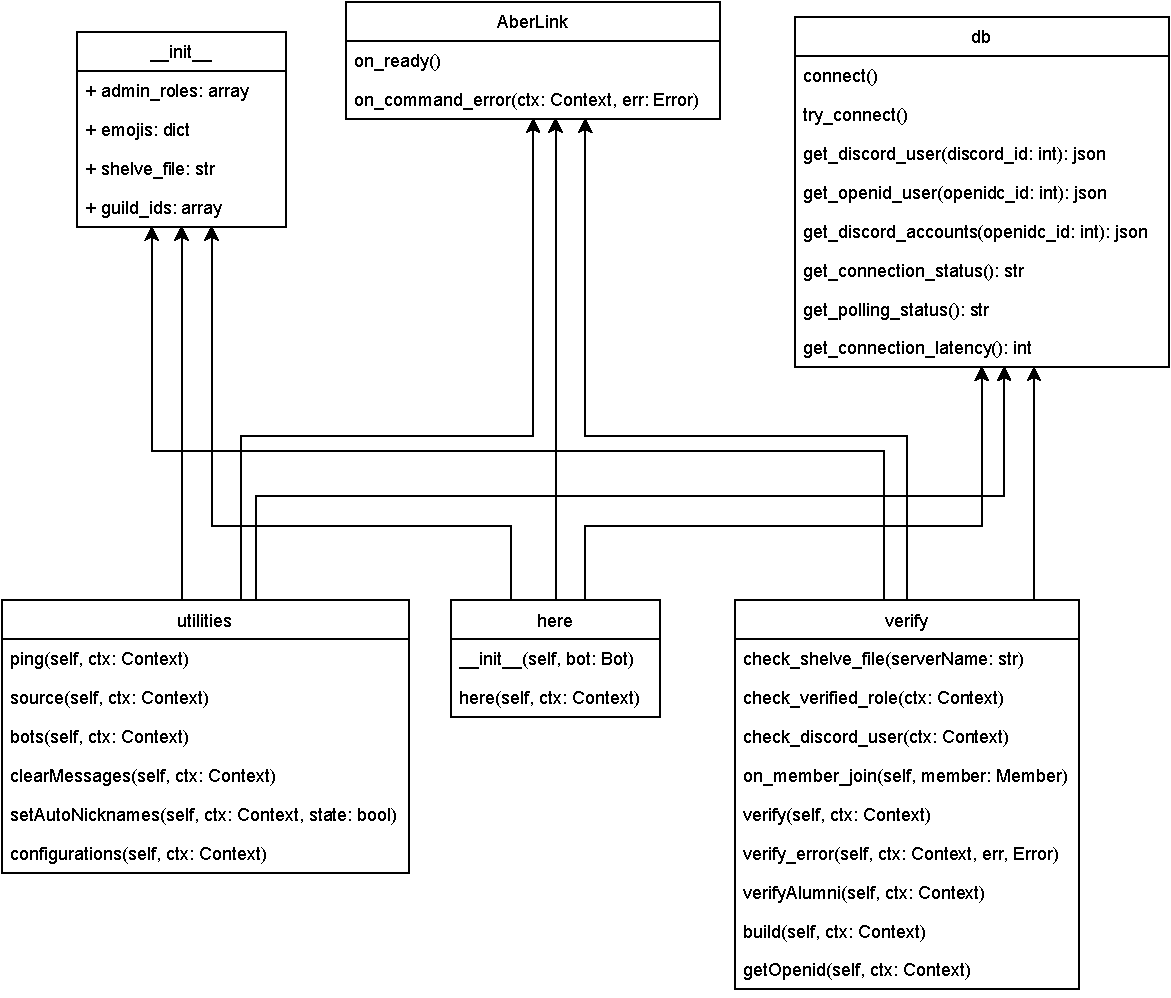
\includegraphics[width=1\linewidth]{Figures/discord-uml}
	\caption{Discord UML diagram}
	\label{fig:discord-uml}
\end{figure}

\subsection{Database Interaction}
Below is a sequence diagram explaining how AberLink connects to database and sends requests back and forth. It uses the Python library psycopg2 to connect and send SQL requests back and forth; the detail of which can be found in the db.py file. Once connected to the database if an error occurs while making a request then the code executes a function (try\_connection()) to reconnect to the database.
\begin{figure}[H]
	\centering
	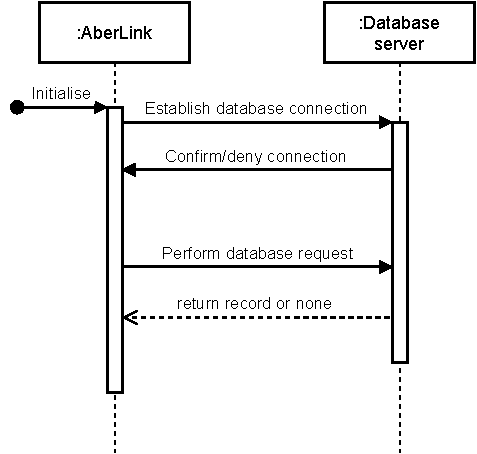
\includegraphics[width=0.5\linewidth]{Figures/aberlink-sequence}
	\caption{Sequence diagram for Discord bot to database}
	\label{fig:architecture-dis-seq}
\end{figure}

\subsection{Complicated Behaviours}
Most of the Discord bot code is relatively straight forward however there is one function in particular that needs some explanation called build() located in /cogs/verify.py. This function and command is used in discord to configure the server for verification and uses the following steps:

\begin{enumerate}
	\item Begins by simulating that the bot is typing
	\item Then searches for the @everyone and verify roles, the verify\_channel
	\item The @everyone role is then stripped of it's permissions entirely so as to stop channel viewing
	\item If the verify role doesn't exist then it is created and it is set with all the default permissions that @everyone used to have
	\item The bot is then given the verify role so that they can view the server channels
	\item If the verify channel doesn't exist then it is created and a message is pinned to the channel asking users to type !verify to verify their accounts
	\item The verify channel then adds the ability for the @everyone role to view and type in the channel to get verified
	\item The verify channel then removes the ability for the verified role to see the channel
	\item Finally once completed the bot stops typing and sends the message "authentication complete"
\end{enumerate}

\section{Database design}
Below is the Entity Relationship diagram that describes how the database works. The tables were created in Django which then remodels the psql \cite{psql} database to fit those requirements. 

\begin{figure}[H]
	\centering
	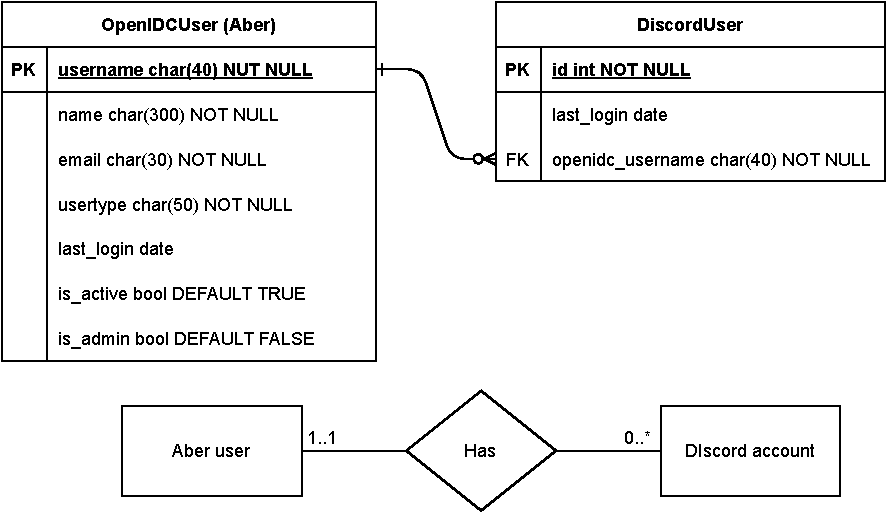
\includegraphics[width=0.8\linewidth]{Figures/database-er-0}
	\caption{Entity relationship diagram for database}
	\label{fig:database-er}
\end{figure}
The \textbf{OpenIDCUser} is the main university account that the user authenticates with and is called so because it uses the OpenID Connect \cite{OpenID} system to authenticate users. The username, name and email are determined from the OpenID Connect response and are all unique. The usertype is also determined by the response and is used to determine if the user will be given administration privileges e.g. if usertype=staff then admin=True. Due to Django's custom user models it requires that the authenticated account has a is\_active column that is kept true unless the account is marked as deactivated.

The \textbf{DiscordUser} is simple and contains a unique Discord id that is a snowflake, a technology invented by twitter to keep id's unique. It also contains a last\_login date to help with possible problems down the line and lastly a openidc\_id that is a foreign key from the OpenIDCUser's id.

Below is an example of the data stored in the database.

\begin{table}[H]
	\centering
	\small
	\setlength\tabcolsep{2pt}
	\begin{tabular}{|c|c|c|c|c|c|c|c|}
		\hline
		\underline{id} & username & name & email & usertype & last\_login & is\_active & is\_admin \\
		\hline
		1 & joa38 & Joel Adams & joa38@aber.ac.uk & staff & datetime & t & t \\
		2 & jet39 & Jenny Thyer & jet39@aber.ac.uk & student & datetime & t & f \\
		3 & maw86 & Michael Antony West & maw86@aber.ac.uk & student & datetime & t & f \\
		\hline 
	\end{tabular}
	\caption{Aberystwyth user table example}
	\label{tab:aber-table}
\end{table}

\begin{table}[H]
	\centering
	\small
	\setlength\tabcolsep{2pt}
	\begin{tabular}{|c|c|c|}
		\hline
		\underline{id}                 & last\_login                   & openidc\_id* \\
		\hline
		727834884915331144 & 2021-02-18 16:43:47.067328+00 & 1           \\
		284352754321719296 & 2021-02-18 16:43:47.067328+00 & 1           \\
		246998944964542464 & 2021-02-04 11:14:40.057891+00 & 2           \\
		282248714955784192 & 2021-02-12 17:35:23.044226+00 & 3           \\
		\hline
	\end{tabular}
	\caption{Discord user table example}
	\label{tab:dis-table}
\end{table}

\section{User Interface}

\subsection{Website}
Before beginning work on the website I designed some website mock-ups that I have used as reference when working on the design of the webpages and are pictured below.
\begin{figure}[H]
	\centering
	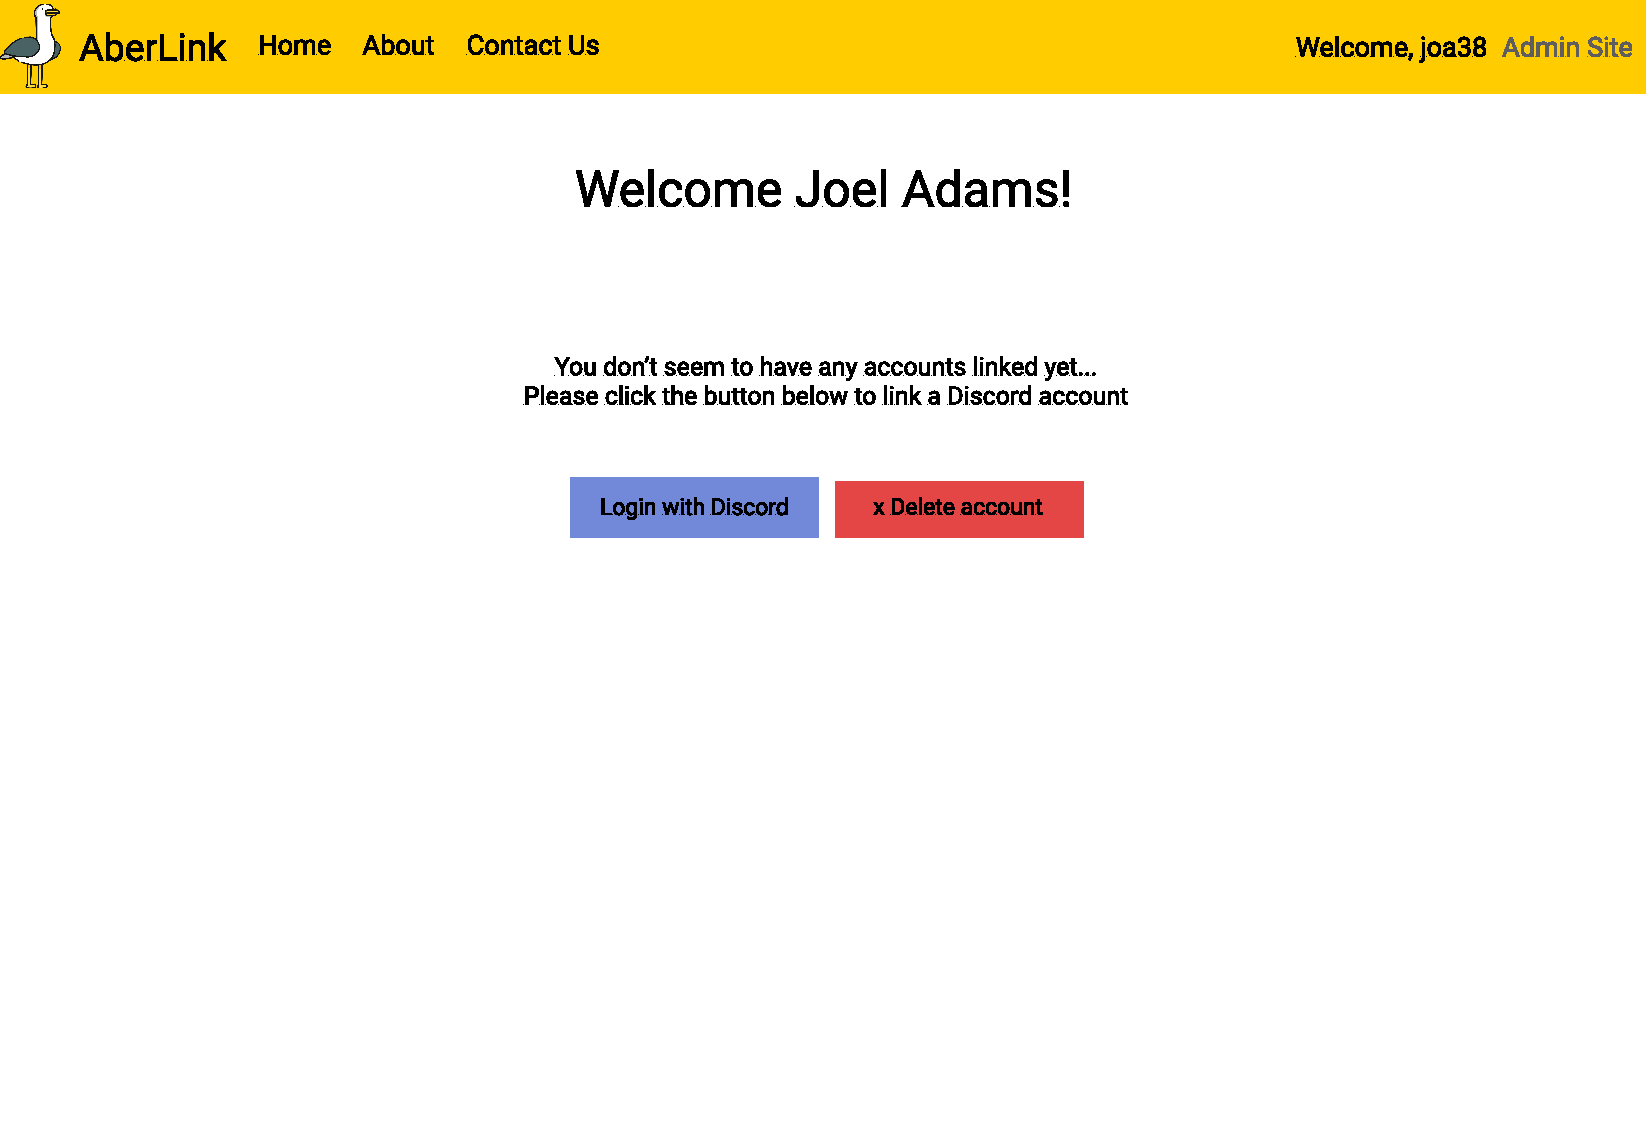
\includegraphics[width=0.8\linewidth]{Figures/AberLink-web-0}
	\caption{Website mock-up for 0 users}
	\label{fig:web-mock-0}
\end{figure}
\begin{figure}[H]
	\centering
	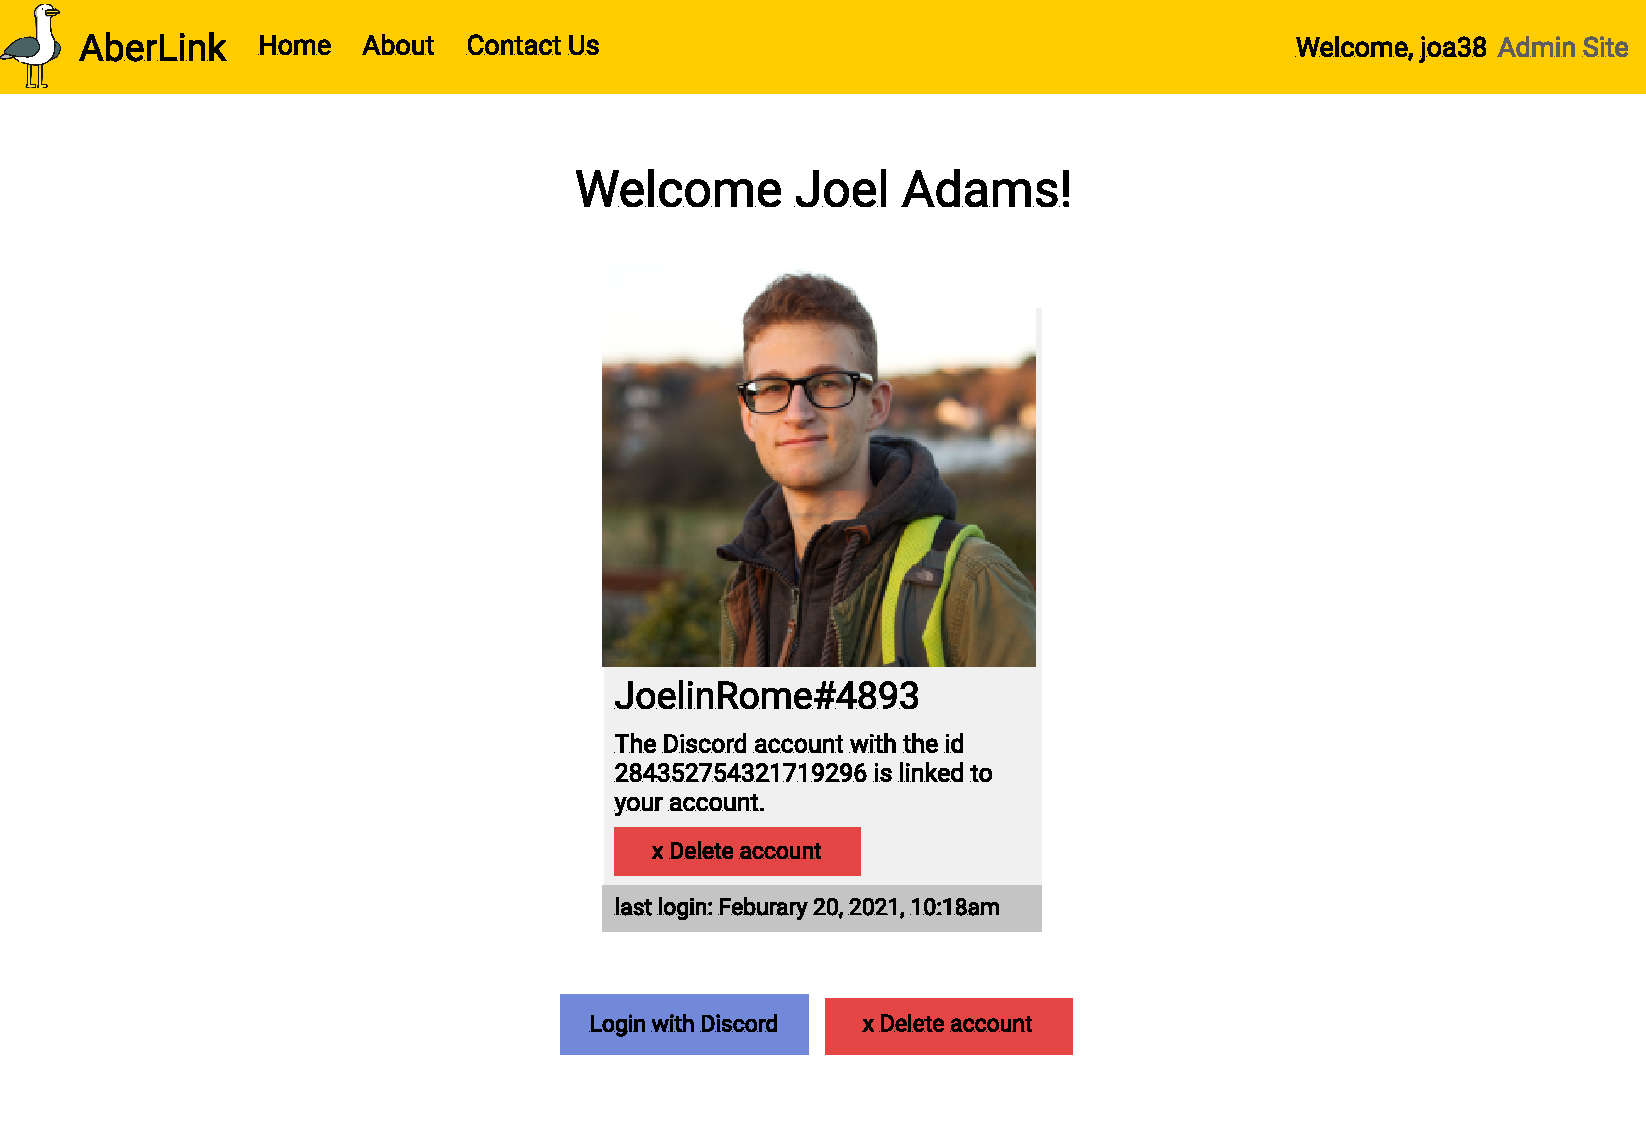
\includegraphics[width=0.8\linewidth]{Figures/AberLink-web-1}
	\caption{Website mock-up for 1 user}
	\label{fig:web-mock-1}
\end{figure}
\begin{figure}[H]
	\centering
	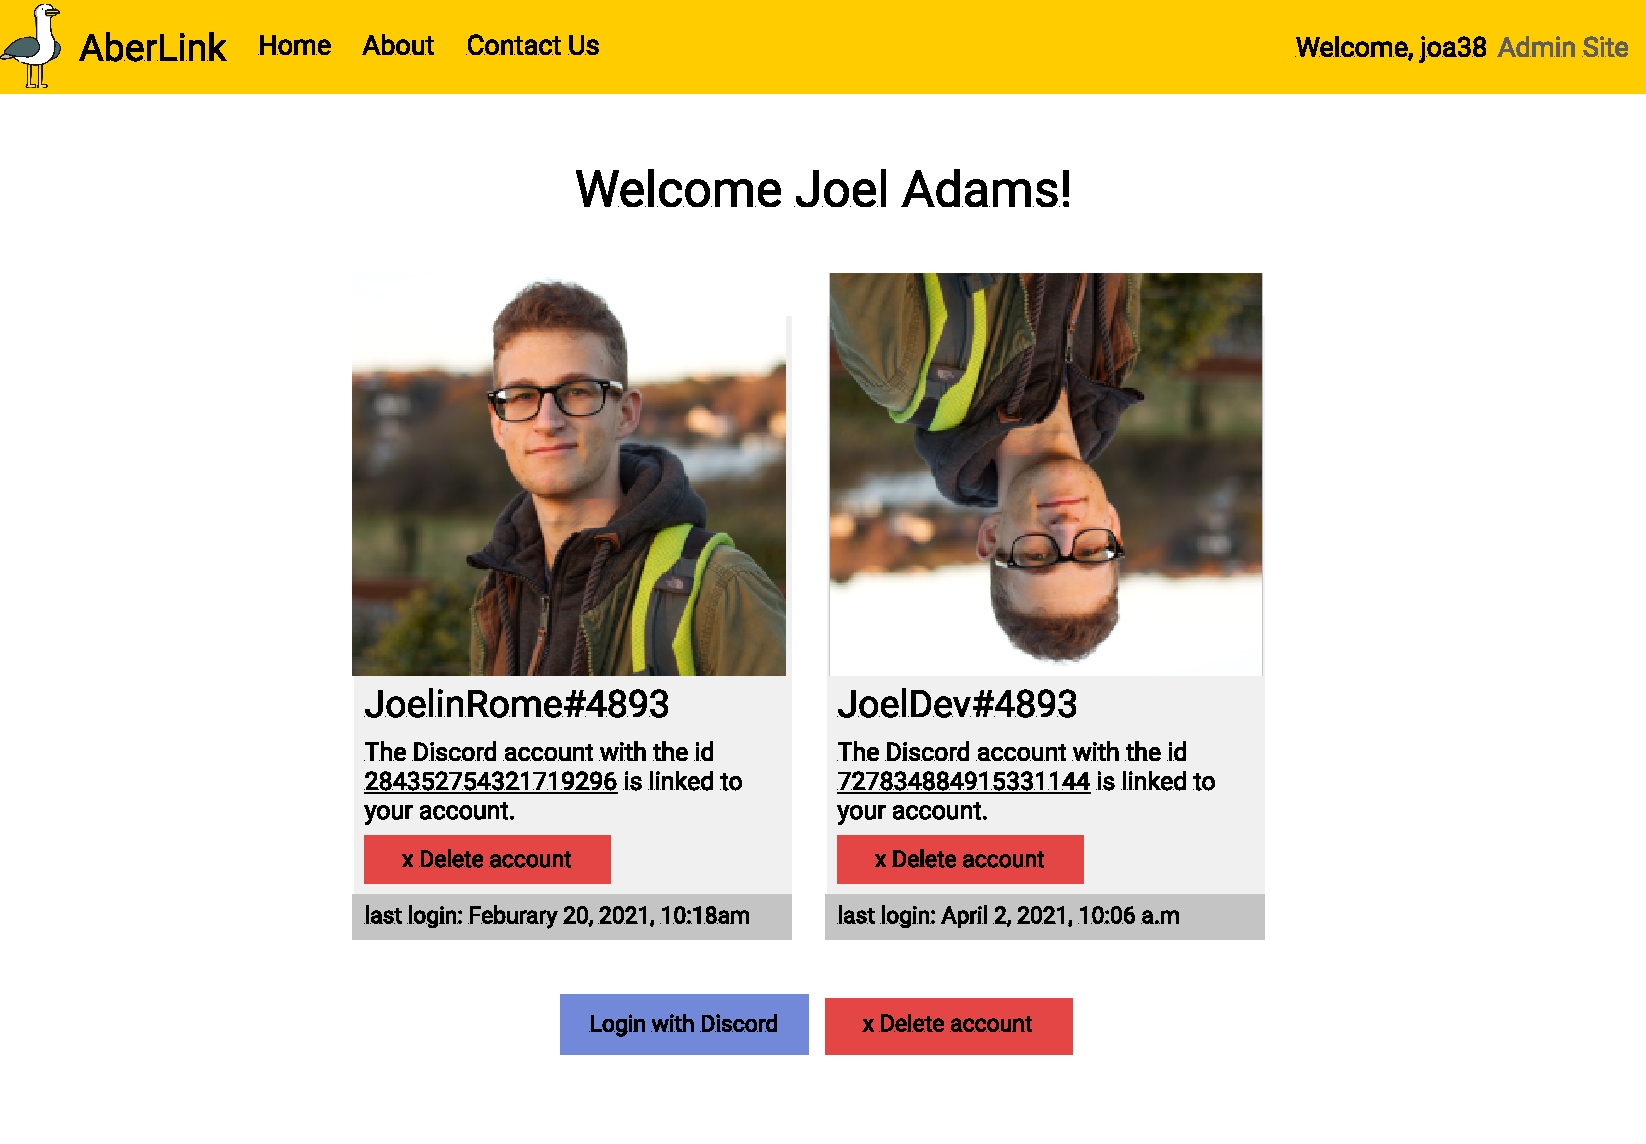
\includegraphics[width=0.8\linewidth]{Figures/AberLink-web-2}
	\caption{Website mock-up for 2 users}
	\label{fig:web-mock-2}
\end{figure}


\subsection{Discord bot}
Discord provides its own interface for Discord bots and doesn't vary much from the regular interface provided to users. Discord bots however have the additional feature of being able to use Embeds which contain far better formatting than regular messages and are used extensively throughout AberLink. Below are some examples of the output of bot commands that I have created.
\begin{figure}[H]
	\centering
	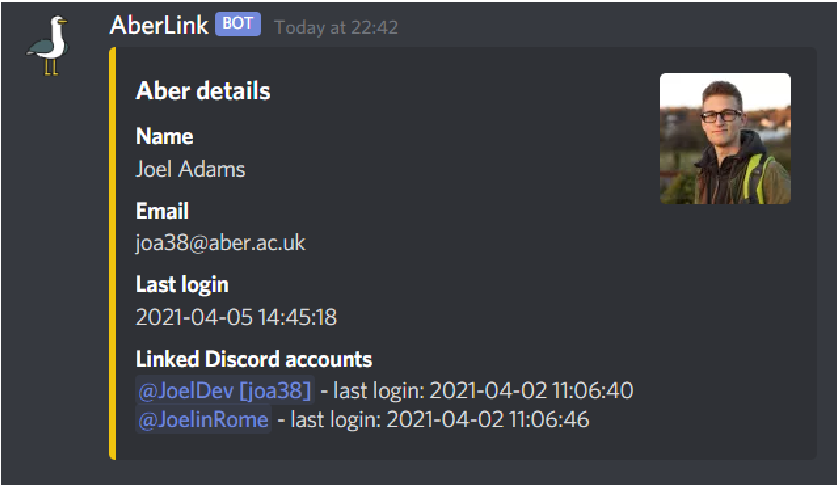
\includegraphics[width=0.8\textwidth]{Figures/test-2}
	\caption{Discord embed example for getting users information}
	\label{fig:dis-go}
\end{figure}
\begin{figure}[H]
	\centering
	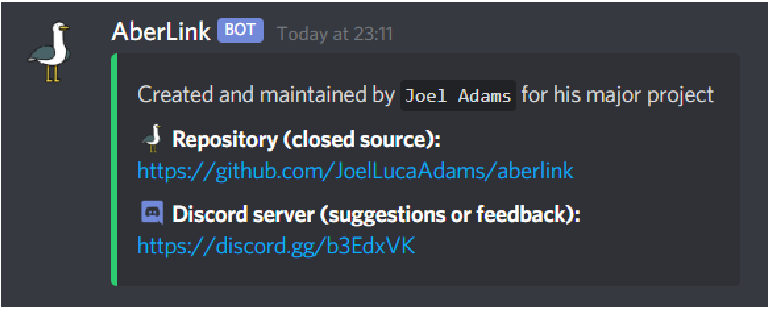
\includegraphics[width=0.8\textwidth]{Figures/test}
	\caption{Discord embed example for source command}
	\label{fig:dis-source}
\end{figure}

